
\documentclass[12pt]{article}
\usepackage[utf8]{inputenc}
\usepackage{geometry}
\usepackage{graphicx}
\usepackage{amsmath}
\usepackage{threeparttable}
\usepackage{hyperref}
\usepackage{lipsum}
%tambahkan package listing untuk kode python dan tambahkan warna agar listing lebih menarik
\usepackage{listings}
\usepackage{float}

\usepackage{xcolor}
\lstset{
    language=Python,
    basicstyle=\ttfamily\small,
    keywordstyle=\color{blue},
    commentstyle=\color{magenta},
    stringstyle=\color{red},
    numbers=left,
    numberstyle=\tiny\color{gray},
    stepnumber=1,
    numbersep=5pt,
    tabsize=4
}
\usepackage{fancyhdr}
\renewcommand{\figurename}{Gambar}
\geometry{margin=1in}

\title{Homework Solution - Unsupervised Learning}
\author{I Gusti Ngurah Agung Hari Vijaya Kusuma Batch 57}
\date{\today}

\begin{document}

\maketitle

\section*{Submission Links}
\begin{itemize}
  \item Repository: \href{https://github.com/AgungHari/Rakamin_HW_UnsupervisedLearning}{github.com/AgungHari}
\end{itemize}

\section{Pendahuluan}
\subsection{Latar Belakang}

Diberikan tugas untuk membuat model unsupervised learning dengan menggunakan dataset yang berisi data customer sebuah perusahaan penerbangan. Dataset ini mencakup berbagai fitur yang dapat menggambarkan nilai dari setiap customer, seperti ID Member, tanggal bergabung dalam program Frequent Flyer, jenis kelamin, tier program, kota asal, provinsi asal, negara asal, umur, jumlah penerbangan yang telah dilakukan, dan informasi terkait jarak penerbangan serta poin yang diperoleh.

Tujuan dari tugas ini adalah untuk menjawab Soal soal yang diberikan oleh Rakamin Academy. Dimana diharapkan outputnya dapat memberikan wawasan yang lebih dalam mengenai pola perilaku customer, segmentasi pasar, dan rekomendasi bisnis yang relevan berdasarkan hasil clustering. Dengan demikian, perusahaan penerbangan dapat mengoptimalkan strategi pemasaran dan meningkatkan pengalaman pelanggan.

\subsection{Homework Unsupervised Learning}

Adapun beberapa soal yang diberikan dalam tugas ini adalah sebagai berikut:
\begin{enumerate}
    \item Lakukan EDA pada dataset untuk mendapatkan pemahaman umum mengenai data dan memandu proses feature engineering (20 poin)
    \begin{itemize}
        \item Pastikan setiap kolom dataset memiliki tipe data yang tepat, tidak ada data kosong, bebas dari duplikat, dan berada di range value yang tepat.
        \item Keluarkan statistik kolom baik numerik maupun kategorikal, cari bentuk distribusi setiap kolom (numerik), dan jumlah baris untuk setiap unique value (kategorikal).
        \item Cari tahu apakah ada kolom-kolom yang berkorelasi kuat satu sama lain.
    \end{itemize}
    
    \item Pilih fitur-fitur yang menurut teman-teman masuk akal secara bisnis untuk digunakan sebagai fitur clustering. Lakukan feature engineering! (20 poin)
    \begin{itemize}
        \item Dari sekian banyak kolom yang ada, tentukan 3-6 fitur untuk digunakan sebagai fitur clustering. Tulis alasan teman-teman memilih fitur tersebut.
        \item Lakukan preprocessing dan feature engineering (apabila fitur yang teman-teman pilih merupakan fitur baru yang dihasilkan dari fitur-fitur yang sudah ada).
    \end{itemize}
    
    \item Lakukan clustering K-means! Temukan jumlah cluster yang menurut teman-teman optimal dan evaluasi cluster yang dihasilkan dengan visualisasi dan silhouette score (30 poin)
    \begin{itemize}
        \item Temukan jumlah cluster yang optimal dengan menggunakan elbow method.
        \item Lakukan clustering menggunakan K-means.
        \item Evaluasi cluster yang dihasilkan dengan menggunakan visualisasi, gunakan PCA apabila diperlukan.
    \end{itemize}
    
    \item Interpretasi cluster yang dihasilkan secara bisnis dan berikan rekomendasi yang sesuai dengan cluster yang dihasilkan (30 poin)
    \begin{itemize}
        \item Tempelkan kembali label yang dihasilkan ke dataframe asal, dan keluarkan statistik fitur dari setiap cluster.
        \item Deskripsikan secara kontekstual customer seperti apa yang ada di masing-masing cluster.
        \item Berdasarkan cluster tersebut, berikan 1-2 rekomendasi bisnis.
    \end{itemize}
\end{enumerate}




\newpage
\section{Tinjauan Pustaka}

% berikut adalah fitur dari dataset buatkan tinjauan pusataka yang merepresentasikan fitur-fitur 
% Code Description
% - MEMBER_NO-b : ID Member
% - FFP_DATE : Frequent Flyer Program Join Date
% - FIRST_FLIGHT_DATE : Tanggal Penerbangan pertama
% - GENDER : Jenis Kelamin
% - FFP_TIER : Tier dari Frequent Flyer Program
% - WORK_CITY : Kota Asal
% - WORK_PROVINCE : Provinsi Asal
% - WORK_COUNTRY : Negara Asal
% - AGE : Umur Customer
% - LOAD_TIME : Tanggal data diambil
% - FLIGHT_COUNT : Jumlah penerbangan Customer
% - BP_SUM : Rencana Perjalanan
% - SUM_YR_1 : Fare Revenue
% - SUM_YR_2 : Votes Prices
% - SEG_KM_SUM : Total jarak(km) penerbangan yg sudah dilakukan
% - LAST_FLIGHT_DATE : Tanggal penerbangan terakhir
% - LAST_TO_END : Jarak waktu penerbangan terakhir ke pesanan penerbangan paling akhir
% - AVG_INTERVAL : Rata-rata jarak waktu
% - MAX_INTERVAL : Maksimal jarak waktu
% - EXCHANGE_COUNT : Jumlah penukaran
% - avg_discount : Rata rata discount yang didapat customer
% - Points_Sum : Jumlah poin yang didapat customer
% - Point_NotFlight : point yang tidak digunakan oleh members

\subsection{Frequent Flyer Program}
Frequent Flyer Program (FFP) adalah program loyalitas yang ditawarkan oleh maskapai penerbangan kepada pelanggan setia mereka. Program ini memberikan berbagai keuntungan, seperti akumulasi poin atau miles yang dapat ditukarkan dengan tiket penerbangan gratis, peningkatan kelas penerbangan, akses ke lounge bandara, dan layanan prioritas lainnya. FFP dirancang untuk mendorong pelanggan agar terus menggunakan layanan maskapai tertentu, sehingga meningkatkan retensi pelanggan dan loyalitas merek.

Program ini biasanya memiliki beberapa tingkatan atau tier, yang memberikan manfaat tambahan kepada anggota yang mencapai tingkat tertentu berdasarkan frekuensi penerbangan atau jumlah poin yang dikumpulkan. Dengan demikian, FFP tidak hanya memberikan insentif bagi pelanggan untuk terbang lebih sering, tetapi juga menciptakan hubungan jangka panjang antara maskapai dan pelanggannya.

\begin{figure}[H]
    \centering
    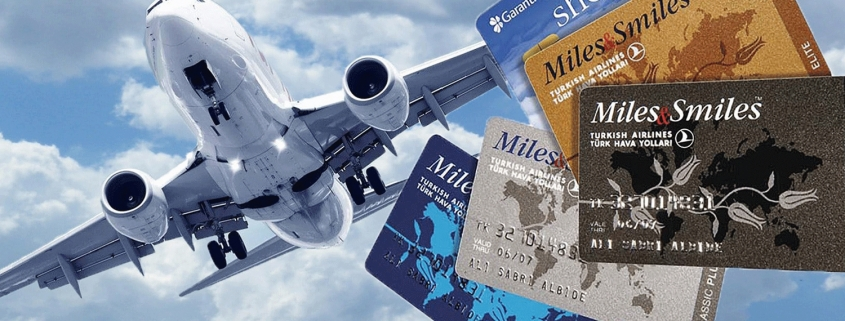
\includegraphics[width=0.6\textwidth]{gambar/ffp.jpg}
    \caption{Contoh Frequent Flyer Program}
    \label{fig:ffp}
\end{figure}

\subsection{EDA (Exploratory Data Analysis)}
Exploratory Data Analysis (EDA) adalah proses analisis data yang bertujuan untuk memahami struktur, pola, dan hubungan dalam dataset sebelum melakukan analisis lebih lanjut atau membangun model. EDA melibatkan penggunaan berbagai teknik statistik dan visualisasi untuk mengeksplorasi data, mengidentifikasi anomali, dan mendapatkan wawasan awal tentang karakteristik data.

Proses EDA biasanya mencakup langkah-langkah seperti:
\begin{itemize}
    \item \textbf{Pemeriksaan Data:} Memeriksa tipe data, nilai yang hilang, dan distribusi variabel.
    \item \textbf{Statistik Deskriptif:} Menghitung ukuran pusat (mean, median) dan ukuran dispersi (standar deviasi, rentang).
    \item \textbf{Visualisasi Data:} Menggunakan grafik seperti histogram, boxplot, dan scatter plot untuk memahami distribusi dan hubungan antar variabel.
    \item \textbf{Identifikasi Outlier:} Mendeteksi nilai-nilai yang tidak biasa yang dapat mempengaruhi analisis.
    \item \textbf{Korelasi:} Menganalisis hubungan antar variabel untuk mengidentifikasi pola yang mungkin ada.
\end{itemize}

EDA sangat penting dalam tahap awal analisis data karena membantu peneliti atau analis untuk memahami data secara mendalam, mengarahkan fokus pada area yang relevan, dan menginformasikan keputusan tentang teknik analisis yang akan digunakan selanjutnya. Dengan demikian, EDA merupakan langkah krusial dalam proses analisis data yang efektif.

\subsection{Data Preprocessing}
Data preprocessing adalah langkah penting dalam analisis data yang melibatkan pembersihan, transformasi, dan persiapan data sebelum digunakan dalam analisis atau pemodelan. Tujuan dari preprocessing adalah untuk memastikan bahwa data dalam kondisi yang baik, konsisten, dan siap untuk dianalisis. Langkah-langkah umum dalam data preprocessing meliputi:
\begin{itemize}
    \item \textbf{Pembersihan Data:} Menghapus atau memperbaiki data yang tidak lengkap, duplikat, atau tidak konsisten. Ini termasuk menangani nilai yang hilang, mengoreksi kesalahan pengetikan, dan menghapus outlier yang tidak relevan.
    \item \textbf{Transformasi Data:} Mengubah format data agar sesuai dengan kebutuhan analisis. Ini bisa meliputi normalisasi atau standarisasi nilai numerik, pengkodean variabel kategorikal, dan konversi tipe data.
    \item \textbf{Penggabungan Data:} Menggabungkan beberapa sumber data menjadi satu dataset yang kohesif, jika diperlukan.
    \item \textbf{Pemisahan Data:} Membagi dataset menjadi subset untuk pelatihan dan pengujian model, terutama dalam konteks machine learning.
    \item \textbf{Feature Engineering:} Membuat fitur baru dari data yang ada untuk meningkatkan kinerja model. Ini bisa meliputi penggabungan variabel, ekstraksi informasi dari teks, atau pembuatan variabel waktu.
    \item \textbf{Skalasi Data:} Mengubah skala fitur numerik agar berada dalam rentang yang sama, yang penting untuk algoritma yang sensitif terhadap skala, seperti K-Means atau SVM.
\end{itemize}

\subsection{K-Means Clustering}
K-Means Clustering adalah algoritma pembelajaran tidak terawasi yang digunakan untuk mengelompokkan data ke dalam sejumlah kluster berdasarkan kesamaan fitur. Algoritma ini bekerja dengan cara membagi dataset menjadi K kluster, di mana setiap kluster diwakili oleh centroid (titik pusat kluster). 
%rumus k-means clustering
Proses K-Means Clustering melibatkan langkah-langkah berikut:
\begin{enumerate}
    \item \textbf{Inisialisasi Centroid:} Memilih K titik acak dari dataset sebagai centroid awal.
    \item \textbf{Penugasan Kluster:} Menghitung jarak antara setiap titik data dan centroid, lalu mengelompokkan setiap titik ke kluster terdekat.
    \item \textbf{Pembaruan Centroid:} Menghitung ulang centroid untuk setiap kluster berdasarkan rata-rata posisi titik-titik dalam kluster tersebut.
    \item \textbf{Iterasi:} Mengulangi langkah 2 dan 3 hingga centroid tidak berubah secara signifikan atau jumlah iterasi maksimum tercapai.
    \item \textbf{Output:} Menghasilkan kluster yang berisi titik-titik data yang dikelompokkan berdasarkan kesamaan fitur.
\end{enumerate}

Adapun rumus untuk menghitung jarak antara titik data dan centroid biasanya menggunakan Euclidean distance, yang didefinisikan sebagai:

\begin{equation}
    d(x, c) = \sqrt{\sum_{i=1}^{n} (x_i - c_i)^2}
\end{equation}
Di mana :
\begin{itemize}
    \item \(d(x, c)\) adalah jarak antara titik data \(x\) dan centroid \(c\),
    \item \(x_i\) adalah nilai fitur ke-i dari titik data \(x\),
    \item \(c_i\) adalah nilai fitur ke-i dari centroid \(c\),
    \item \(n\) adalah jumlah fitur.
    \item \(x\) adalah titik data yang akan dikelompokkan.
    \item \(c\) adalah centroid dari kluster yang sedang dianalisis.
\end{itemize}

K-Means Clustering banyak digunakan dalam berbagai aplikasi, seperti segmentasi pasar, pengelompokan dokumen, dan analisis citra. Kelebihan dari algoritma ini adalah kesederhanaannya dan efisiensi dalam menangani dataset besar. Namun, K-Means juga memiliki beberapa kelemahan, seperti ketergantungan pada pemilihan jumlah kluster \(K\) yang tepat dan sensitivitas terhadap outlier.

\subsection{Elbow Method}
Elbow Method adalah teknik yang digunakan untuk menentukan jumlah optimal kluster \(K\) dalam algoritma K-Means Clustering. Metode ini melibatkan pengukuran varians dalam kluster (inertia) untuk berbagai nilai \(K\) dan kemudian memplot hasilnya. Tujuan dari Elbow Method adalah untuk menemukan titik di mana penambahan kluster baru tidak memberikan peningkatan signifikan dalam pengurangan varians.

Proses Elbow Method meliputi langkah-langkah berikut:
\begin{enumerate}
    \item \textbf{Inisialisasi K-Means:} Jalankan algoritma K-Means untuk berbagai nilai \(K\) (misalnya, dari 1 hingga 10).
    \item \textbf{Hitung Inertia:} Untuk setiap nilai \(K\), hitung inertia, yaitu jumlah jarak kuadrat antara titik data dan centroid kluster mereka.
    \item \textbf{Plot Inertia:} Buat plot dengan nilai \(K\) pada sumbu x dan inertia pada sumbu y.
    \item \textbf{Identifikasi Elbow:} Cari titik di mana penurunan inertia mulai melambat, yang biasanya terlihat seperti "siku" pada plot. Titik ini menunjukkan jumlah kluster optimal.
    \item \textbf{Pilih K Optimal:} Nilai \(K\) pada titik siku ini dianggap sebagai jumlah kluster yang paling sesuai untuk dataset.
\end{enumerate}

Elbow Method membantu dalam menghindari overfitting dengan memilih jumlah kluster yang tepat, sehingga model K-Means dapat menangkap struktur data dengan baik tanpa menjadi terlalu kompleks. Meskipun metode ini sederhana dan intuitif, hasilnya dapat bervariasi tergantung pada dataset dan distribusi data, sehingga penting untuk mempertimbangkan konteks analisis saat menentukan jumlah kluster optimal.

\subsection{Silhouette Score}
Silhouette Score adalah metrik yang digunakan untuk mengevaluasi kualitas klustering dalam algoritma K-Means atau metode klustering lainnya. Metrik ini mengukur seberapa baik setiap titik data dikelompokkan dalam kluster yang benar, dengan mempertimbangkan jarak antar titik dalam kluster dan jarak ke titik di kluster lain.
Silhouette Score untuk setiap titik data dihitung dengan rumus berikut:

\begin{equation}
    s(i) = \frac{b(i) - a(i)}{\max(a(i), b(i))}
\end{equation}

Di mana:
\begin{itemize}
    \item \(s(i)\) adalah Silhouette Score untuk titik data \(i\),
    \item \(a(i)\) adalah rata-rata jarak antara titik data \(i\) dan semua titik lain dalam kluster yang sama (intra-kluster),
    \item \(b(i)\) adalah rata-rata jarak antara titik data \(i\) dan titik-titik di kluster terdekat lainnya (inter-kluster).
    \item \(i\) adalah indeks dari titik data yang sedang dianalisis.
\end{itemize}

Nilai Silhouette Score berkisar antara -1 hingga 1:
\begin{itemize}
    \item Nilai mendekati 1 menunjukkan bahwa titik data berada jauh dari kluster lain dan dekat dengan kluster yang benar.
    \item Nilai mendekati 0 menunjukkan bahwa titik data berada di batas antara dua kluster.
    \item Nilai negatif menunjukkan bahwa titik data mungkin telah dikelompokkan ke kluster yang salah.
\end{itemize}

Silhouette Score memberikan gambaran tentang seberapa baik klustering dilakukan, dengan nilai yang lebih tinggi menunjukkan klustering yang lebih baik. Metrik ini berguna untuk membandingkan hasil klustering dengan jumlah kluster yang berbeda dan membantu dalam memilih jumlah kluster yang optimal.

\subsection{PCA (Principal Component Analysis)}
Principal Component Analysis (PCA) adalah teknik reduksi dimensi yang digunakan untuk mengurangi jumlah variabel dalam dataset sambil mempertahankan sebanyak mungkin informasi yang ada. PCA bekerja dengan mengidentifikasi arah (komponen utama) di mana data memiliki varians terbesar, sehingga memungkinkan representasi data dalam ruang dimensi yang lebih rendah.

Proses PCA melibatkan langkah-langkah berikut:
\begin{enumerate}
    \item \textbf{Standardisasi Data:} Mengubah data sehingga memiliki rata-rata 0 dan deviasi standar 1 untuk setiap fitur, agar setiap fitur berkontribusi secara setara.
    \item \textbf{Kovarians Matriks:} Menghitung matriks kovarians untuk memahami hubungan antar fitur dalam dataset.
    \item \textbf{Eigen Decomposition:} Menghitung nilai eigen (eigenvalues) dan vektor eigen (eigenvectors) dari matriks kovarians. Vektor eigen menunjukkan arah komponen utama, sedangkan nilai eigen menunjukkan seberapa banyak varians yang dijelaskan oleh masing-masing komponen.
    \item \textbf{Pemilihan Komponen Utama:} Memilih sejumlah komponen utama berdasarkan nilai eigen terbesar, yang akan digunakan untuk merepresentasikan data dalam dimensi yang lebih rendah.
    \item \textbf{Transformasi Data:} Mengalikan data asli dengan vektor eigen terpilih untuk mendapatkan representasi baru dalam ruang dimensi yang lebih rendah.
\end{enumerate}

PCA sangat berguna dalam mengurangi kompleksitas data, menghilangkan redundansi, dan meningkatkan efisiensi komputasi dalam analisis data. Selain itu, PCA juga membantu dalam visualisasi data dengan mengurangi dimensi menjadi 2 atau 3 komponen utama, sehingga memudahkan pemahaman pola dan struktur dalam dataset. Namun, penting untuk diingat bahwa PCA adalah teknik linier, sehingga mungkin tidak cocok untuk semua jenis data, terutama yang memiliki hubungan non-linier yang kompleks.

\subsection{RFM (Recency, Frequency, Monetary)}
RFM (Recency, Frequency, Monetary) adalah metode analisis yang digunakan untuk mengukur nilai pelanggan berdasarkan tiga dimensi utama:

\begin{itemize}
    \item \textbf{Recency (R):} Mengukur seberapa baru pelanggan melakukan pembelian. Semakin baru pembelian, semakin tinggi nilai recency.
    \item \textbf{Frequency (F):} Mengukur seberapa sering pelanggan melakukan pembelian dalam periode tertentu. Semakin sering pembelian, semakin tinggi nilai frequency.
    \item \textbf{Monetary (M):} Mengukur total pengeluaran pelanggan dalam periode tertentu. Semakin besar pengeluaran, semakin tinggi nilai monetary.
\end{itemize}






\newpage
\section{Desain dan Implementasi}
% buat penjelasan tentang desain dan implementasi sistem untuk membuat model unsupervised learning untuk clustering customer airline frequent flyer program
Pada bab ini, akan dijelaskan mengenai desain dan implementasi sistem yang digunakan untuk membuat model unsupervised learning dalam melakukan clustering terhadap customer airline frequent flyer program. Sistem ini bertujuan untuk mengelompokkan customer berdasarkan karakteristik dan perilaku mereka dalam menggunakan layanan penerbangan, sehingga dapat membantu perusahaan dalam memahami kebutuhan dan preferensi pelanggan.


\subsection{Deskripsi sistem}
Sistem yang dibangun menggunakan data dari frequent flyer program yang berisi informasi mengenai customer airline. Data ini mencakup berbagai atribut seperti ID member, tanggal bergabung dengan program, jenis kelamin, tier program, kota dan provinsi asal, umur, jumlah penerbangan, total jarak penerbangan, dan informasi lainnya yang relevan. Namun sebelum itu data yang digunakan harus melalui proses cleaning, transformasi, dan normalisasi untuk memastikan kualitas data yang baik. Agar tugas clustering dapat dilakukan dengan efektif, maka diperlukan alur kerja yang sistematis. Gambar \ref{fig:flowchart} menunjukkan alur kerja sistem yang digunakan dalam tugas ini.

\begin{figure}[H]
    \centering
    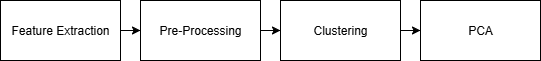
\includegraphics[width=0.8\textwidth]{gambar/flowchart.png}
    \caption{Alur kerja sistem}
    \label{fig:flowchart}
\end{figure}

\subsection{Deskripsi Data}
% Code Description
% - MEMBER_NO-b : ID Member
% - FFP_DATE : Frequent Flyer Program Join Date
% - FIRST_FLIGHT_DATE : Tanggal Penerbangan pertama
% - GENDER : Jenis Kelamin
% - FFP_TIER : Tier dari Frequent Flyer Program
% - WORK_CITY : Kota Asal
% - WORK_PROVINCE : Provinsi Asal
% - WORK_COUNTRY : Negara Asal
% - AGE : Umur Customer
% - LOAD_TIME : Tanggal data diambil
% - FLIGHT_COUNT : Jumlah penerbangan Customer
% - BP_SUM : Rencana Perjalanan
% - SUM_YR_1 : Fare Revenue
% - SUM_YR_2 : Votes Prices
% - SEG_KM_SUM : Total jarak(km) penerbangan yg sudah dilakukan
% - LAST_FLIGHT_DATE : Tanggal penerbangan terakhir
% - LAST_TO_END : Jarak waktu penerbangan terakhir ke pesanan penerbangan paling akhir
% - AVG_INTERVAL : Rata-rata jarak waktu
% - MAX_INTERVAL : Maksimal jarak waktu
% - EXCHANGE_COUNT : Jumlah penukaran
% - avg_discount : Rata rata discount yang didapat customer
% - Points_Sum : Jumlah poin yang didapat customer
% - Point_NotFlight : point yang tidak digunakan oleh members

Data yang digunakan dalam sistem ini merupakan data dari frequent flyer program yang berisi informasi mengenai customer airline. Berikut adalah deskripsi dari atribut-atribut yang terdapat dalam dataset :

\begin{itemize}
    \item \textbf{MEMBER\_NO}: ID unik untuk setiap member.
    \item \textbf{FFP\_DATE}: Tanggal bergabung dengan frequent flyer program.
    \item \textbf{FIRST\_FLIGHT\_DATE}: Tanggal penerbangan pertama yang dilakukan oleh member.
    \item \textbf{GENDER} :Jenis kelamin dari member (Laki-laki atau Perempuan).
    \item \textbf{FFP\_TIER}: Tier dari frequent flyer program yang diikuti oleh member (misalnya Silver, Gold, Platinum).
    \item \textbf{WORK\_CITY}: Kota asal member.
    \item \textbf{WORK\_PROVINCE}: Provinsi asal member.
    \item \textbf{WORK\_COUNTRY}: Negara asal member.
    \item \textbf{AGE}: Umur customer pada saat data diambil.
    \item \textbf{LOAD\_TIME}: Tanggal dan waktu ketika data diambil.
    \item \textbf{FLIGHT\_COUNT}: Jumlah penerbangan yang telah dilakukan oleh customer.
    \item \textbf{BP\_SUM}: Rencana perjalanan yang telah dilakukan oleh customer.
    \item \textbf{SUM\_YR\_1}: Total fare revenue yang dihasilkan oleh customer pada tahun pertama.
    \item \textbf{SUM\_YR\_2}: Total fare revenue yang dihasilkan oleh customer pada tahun kedua.
    \item \textbf{SEG\_KM\_SUM}: Total jarak (dalam kilometer) penerbangan yang telah dilakukan oleh customer.
    \item \textbf{LAST\_FLIGHT\_DATE}: Tanggal penerbangan terakhir yang dilakukan oleh customer.
    \item \textbf{LAST\_TO\_END}: Jarak waktu antara penerbangan terakhir dengan pesanan penerbangan paling akhir.
    \item \textbf{AVG\_INTERVAL}: Rata-rata jarak waktu antara penerbangan yang dilakukan oleh customer.
    \item \textbf{MAX\_INTERVAL}: Maksimal jarak waktu antara penerbangan yang dilakukan oleh customer.
    \item \textbf{EXCHANGE\_COUNT}: Jumlah penukaran yang dilakukan oleh customer.
    \item \textbf{avg\_discount}: Rata-rata diskon yang didapatkan oleh customer.
    \item \textbf{Points\_Sum}: Jumlah poin yang didapatkan oleh customer dari frequent flyer program.
    \item \textbf{Point\_NotFlight}: Poin yang tidak digunakan oleh members, biasanya poin ini bisa digunakan untuk berbagai keperluan seperti upgrade kelas penerbangan atau penukaran dengan barang.
    \item \textbf{Points\_Sum}: Jumlah total poin yang telah dikumpulkan oleh customer dari frequent flyer program.
    \item \textbf{Point\_NotFlight}: Poin yang tidak digunakan oleh members, biasanya poin ini bisa digunakan untuk berbagai keperluan seperti upgrade kelas penerbangan atau penukaran dengan barang.
\end{itemize}

\subsection{Feature Extraction}
% Feature Extraction
Dalam tugas ini, agar model unsupervised learning dapat bekerja dengan baik, perlu dilakukan feature extraction untuk memilih atribut-atribut yang relevan dari dataset. Atribut-atribut yang dipilih harus mampu merepresentasikan karakteristik dan perilaku customer dalam menggunakan layanan penerbangan. Agar mendapatkan fitur fitur yang relevan maka perlu dilakukan analisis terhadap data yang ada. Diharapkan dengan analisa analisa tersebut, fitur yang dihasilkan dapat memberikan informasi yang cukup untuk melakukan clustering terhadap customer airline frequent flyer program.

\subsection{EDA (Exploratory Data Analysis)}
% EDA
Exploratory Data Analysis (EDA) dilakukan untuk memahami karakteristik data yang ada, menemukan pola, dan mengidentifikasi hubungan antar atribut. EDA juga membantu dalam mendeteksi adanya missing values, outliers, dan distribusi data. Beberapa teknik yang digunakan dalam EDA antara lain visualisasi data menggunakan grafik, analisis statistik deskriptif, dan pengelompokan data berdasarkan atribut tertentu.

Namun sebelum melakukan EDA, perlu dilakukan beberapa tahap persiapan data seperti penyesuaian tipe data, penghapusan duplikasi, dan penanganan missing values. Setelah data siap, EDA dapat dilakukan dengan menggunakan berbagai teknik visualisasi seperti histogram, boxplot, scatter plot, dan heatmap untuk melihat hubungan antar atribut.

\subsubsection{Data Cleaning}
% Data Cleaning
Data cleaning adalah proses penting dalam persiapan data sebelum melakukan analisis. Proses ini meliputi penghapusan duplikasi, penanganan missing values, dan penyesuaian tipe data. Dalam tugas ini, data yang digunakan telah melalui proses cleaning untuk memastikan kualitas data yang baik. Berikut merupakan jumlah missing values pada setiap atribut yang ada pada dataset, lstlisting berikut merupakan output cell dari notebook yang menampilkan jumlah missing values pada setiap atribut:

\begin{lstlisting}[language=Python]
# Menampilkan jumlah missing values pada setiap atribut
missing_values = df.isnull().sum()

# output
MEMBER_NO               0
FFP_DATE                0
FIRST_FLIGHT_DATE       0
GENDER                  3
FFP_TIER                0
WORK_CITY            2269
WORK_PROVINCE        3248
WORK_COUNTRY           26
AGE                   420
LOAD_TIME               0
FLIGHT_COUNT            0
BP_SUM                  0
SUM_YR_1              551
SUM_YR_2              138
SEG_KM_SUM              0
LAST_FLIGHT_DATE        0
LAST_TO_END             0
AVG_INTERVAL            0
MAX_INTERVAL            0
EXCHANGE_COUNT          0
avg_discount            0
Points_Sum              0
Point_NotFlight         0
dtype: int64
\end{lstlisting}

Dapat dilihat bahwa 5.15\% missing value dari keseluruhan data, karena jumlahnya cukup kecil saya memutuskan untuk membuang data yang memiliki missing value, hal ini dilakukan untuk menjaga kualitas data yang akan digunakan dalam proses clustering. Setelah proses data cleaning selesai, data siap digunakan untuk analisis lebih lanjut.

\subsubsection{Handle Duplikat}
% Handle Duplikat
Setelah proses data cleaning, langkah selanjutnya adalah menangani duplikasi data. Duplikasi dapat terjadi ketika ada beberapa entri yang memiliki informasi yang sama. Dalam tugas ini, saya melakukan pengecekan terhadap duplikasi data dengan menggunakan fungsi \texttt{duplicated()} pada DataFrame. Jika ditemukan duplikasi, maka entri tersebut akan dihapus untuk memastikan bahwa setiap customer hanya memiliki satu entri dalam dataset.

\begin{lstlisting}[language=Python]
    # Print jumlah data duplikat
    print("Jumlah data duplikat:", df.duplicated().sum())

    # Output
    Jumlah data duplikat: 0
\end{lstlisting}

Setelah melakukan pengecekan, ternyata tidak ditemukan data duplikat dalam dataset. Hal ini menunjukkan bahwa setiap customer memiliki entri yang unik, sehingga data siap digunakan untuk analisis lebih lanjut.

\newpage

\subsubsection{Handle Tipe Data}
% Handle Tipe Data
Setelah proses data cleaning dan penanganan duplikasi, langkah selanjutnya adalah memastikan bahwa tipe data pada setiap atribut sesuai dengan yang diharapkan. Hal ini penting untuk memastikan bahwa analisis yang dilakukan dapat berjalan dengan baik. Dalam tugas ini, saya melakukan pengecekan terhadap tipe data pada setiap atribut menggunakan fungsi \texttt{dtypes} pada DataFrame.

\begin{lstlisting}[language=Python]
# Print tipe data pada setiap atribut
df.info

# Output
class 'pandas.core.frame.DataFrame'>
RangeIndex: 62988 entries, 0 to 62987
Data columns (total 23 columns):
 #   Column             Non-Null Count  Dtype  
---  ------             --------------  -----  
 0   MEMBER_NO          62988 non-null  int64  
 1   FFP_DATE           62988 non-null  object 
 2   FIRST_FLIGHT_DATE  62988 non-null  object 
.....
.....
 22  Point_NotFlight    62988 non-null  int64  
 23  Points_Sum         62988 non-null  int64
\end{lstlisting}

Dari hasil pengecekan, dapat dilihat bahwa beberapa atribut memiliki tipe data yang tidak sesuai, terutama untuk data yang seharusnya bertipe tanggal. Oleh karena itu, saya melakukan konversi tipe data pada atribut-atribut tersebut menjadi tipe data yang sesuai, seperti mengubah atribut \texttt{FFP\_DATE} dan \texttt{FIRST\_FLIGHT\_DATE} menjadi tipe data \texttt{datetime}. Hal ini dilakukan untuk memastikan bahwa analisis yang dilakukan dapat berjalan dengan baik dan menghasilkan informasi yang akurat.

\subsubsection{Analisis Fitur Numerikal}
% Analisis Fitur Numerikal
Setelah proses data cleaning dan penanganan tipe data, langkah selanjutnya adalah melakukan analisis terhadap fitur numerikal yang ada dalam dataset. Fitur numerikal adalah atribut yang memiliki nilai numerik dan dapat digunakan untuk analisis statistik. Dalam tugas ini, saya melakukan analisis dengan menggunakan boxplot untuk melihat distribusi data dan mendeteksi adanya outliers pada fitur numerikal. Boxplot memberikan gambaran yang jelas mengenai nilai minimum, maksimum, median, dan kuartil dari setiap fitur numerikal. Gambar \ref{fig:boxplot} menunjukkan boxplot dari fitur numerikal yang ada dalam dataset.

\begin{figure}[H]
    \centering
    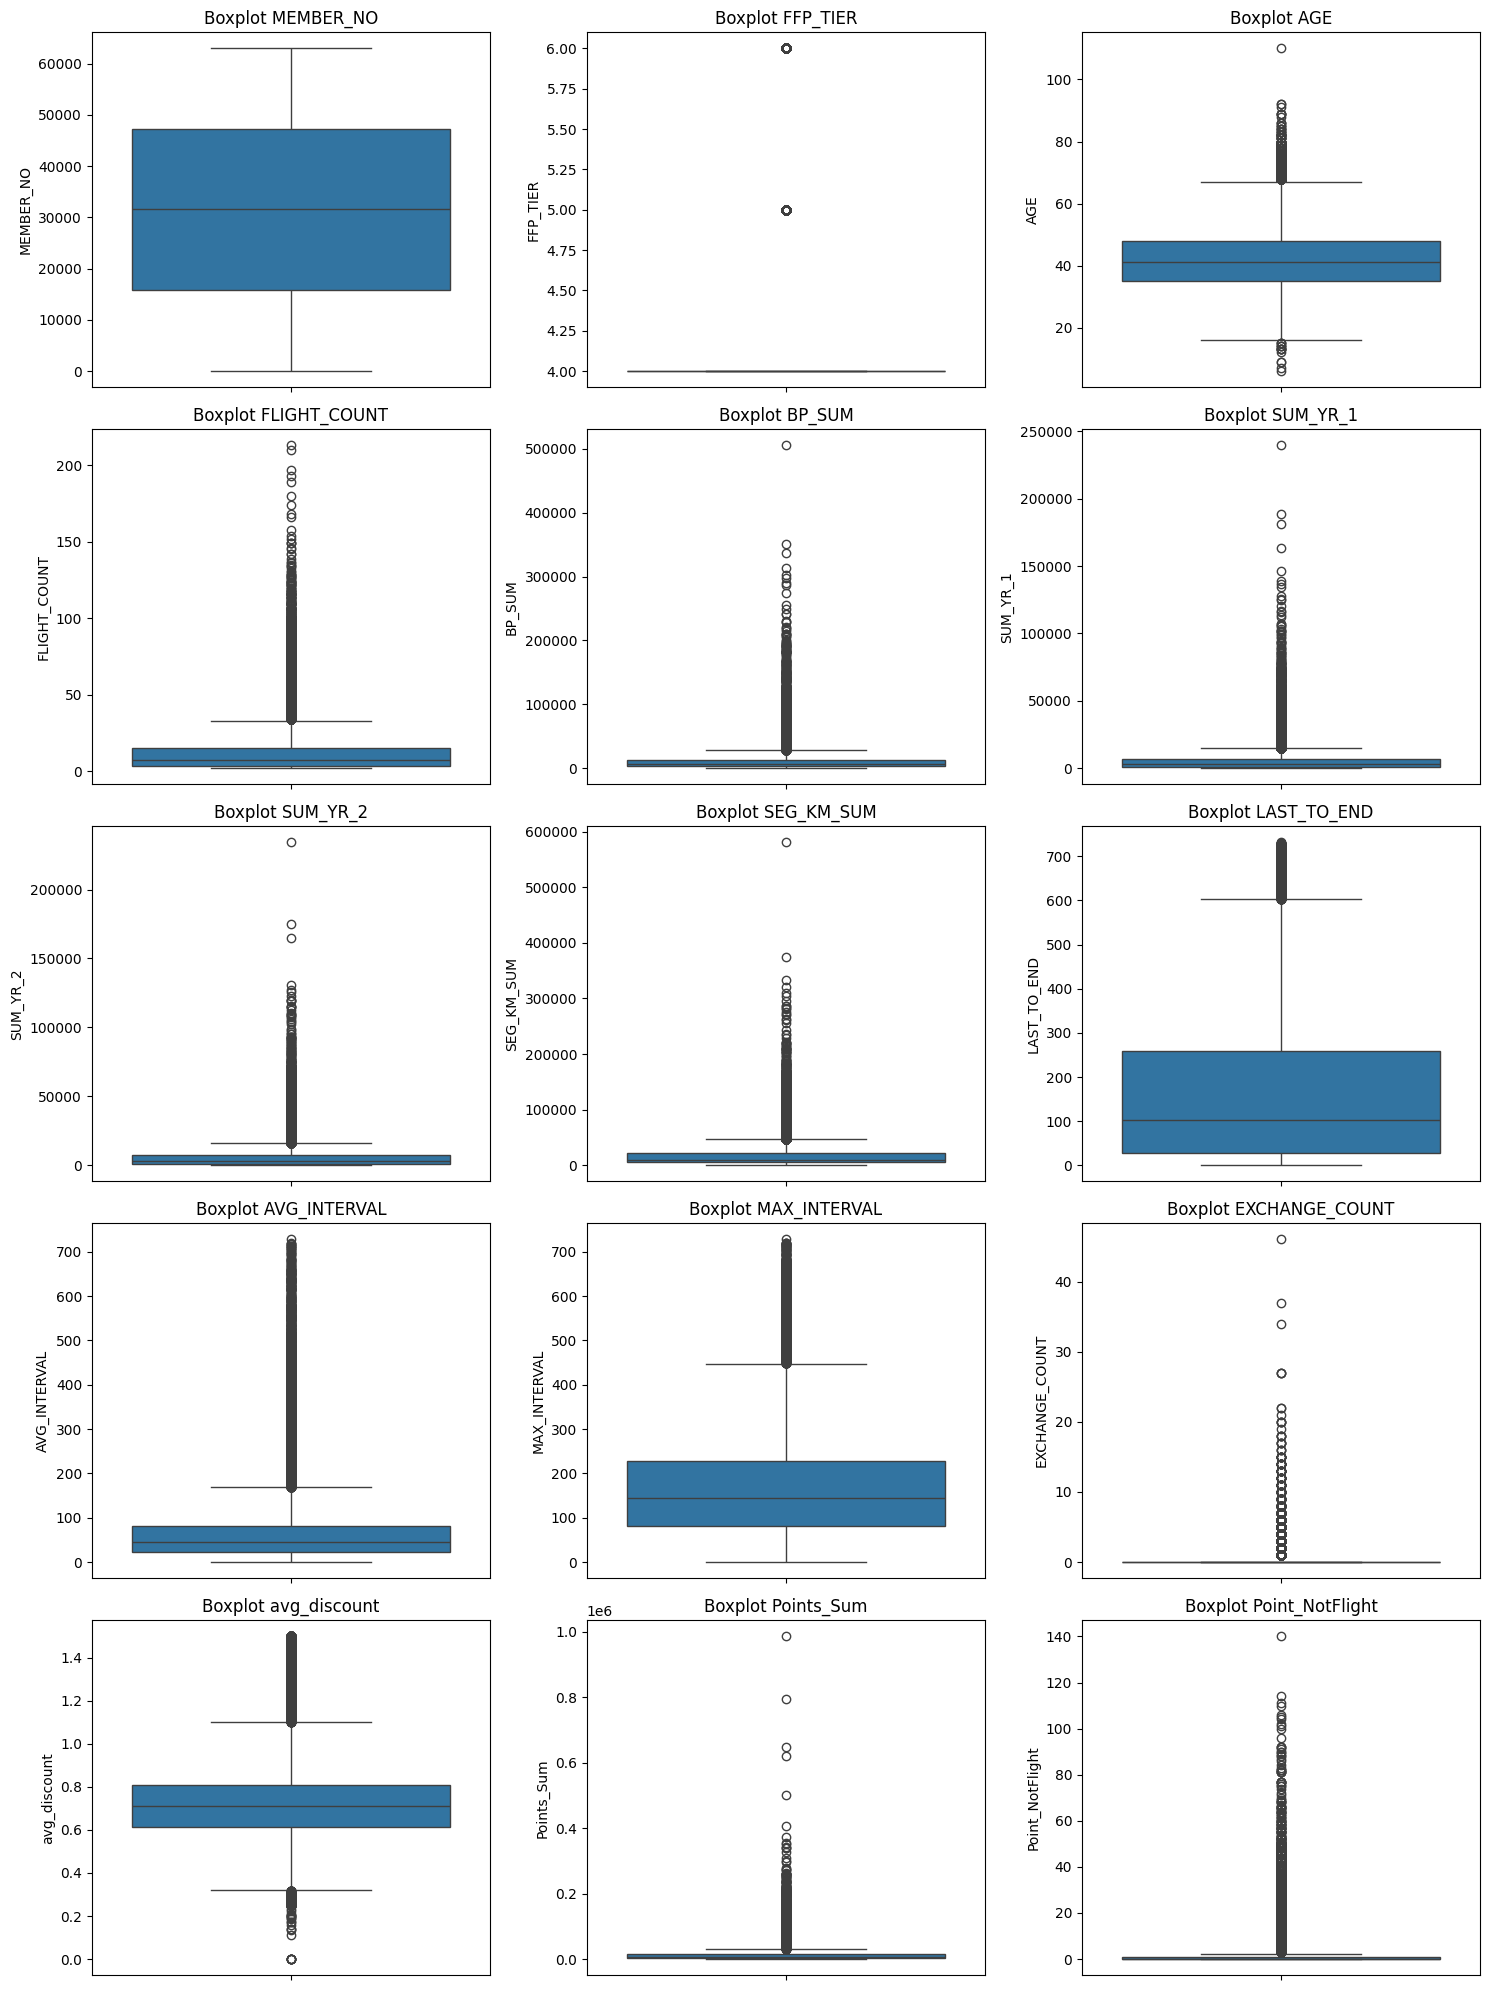
\includegraphics[width=0.7\textwidth]{gambar/boxplot.png}
    \caption{Boxplot dari fitur numerikal}
    \label{fig:boxplot}
\end{figure}

Dari boxplot tersebut, dapat dilihat bahwa beberapa fitur memiliki outliers yang cukup signifikan, dan bahkan ada beberapa yang extreme. Hal ini menunjukkan bahwa ada beberapa customer yang memiliki karakteristik yang berbeda dari mayoritas customer lainnya. Outliers ini perlu diperhatikan dalam proses clustering, karena dapat mempengaruhi hasil clustering yang dihasilkan. Didasari oleh temuan ini saya memutuskan untuk melakukan penanganan terhadap outliers dengan metode IQR (Interquartile Range). Metode ini akan membantu dalam mengidentifikasi dan menangani outliers yang extreme, sehingga data yang digunakan untuk clustering menjadi lebih representatif. Namun sebelum itu kita akan melihat korelasi antar fitur numerikal yang ada pada dataset.

Untuk melihat korelasi antar fitur numerikal, saya menggunakan heatmap yang menunjukkan hubungan antar fitur. Heatmap memberikan gambaran yang jelas mengenai seberapa kuat hubungan antara satu fitur dengan fitur lainnya. Gambar \ref{fig:heatmap} menunjukkan heatmap dari fitur numerikal yang ada dalam dataset.

\begin{figure}[H]
    \centering
    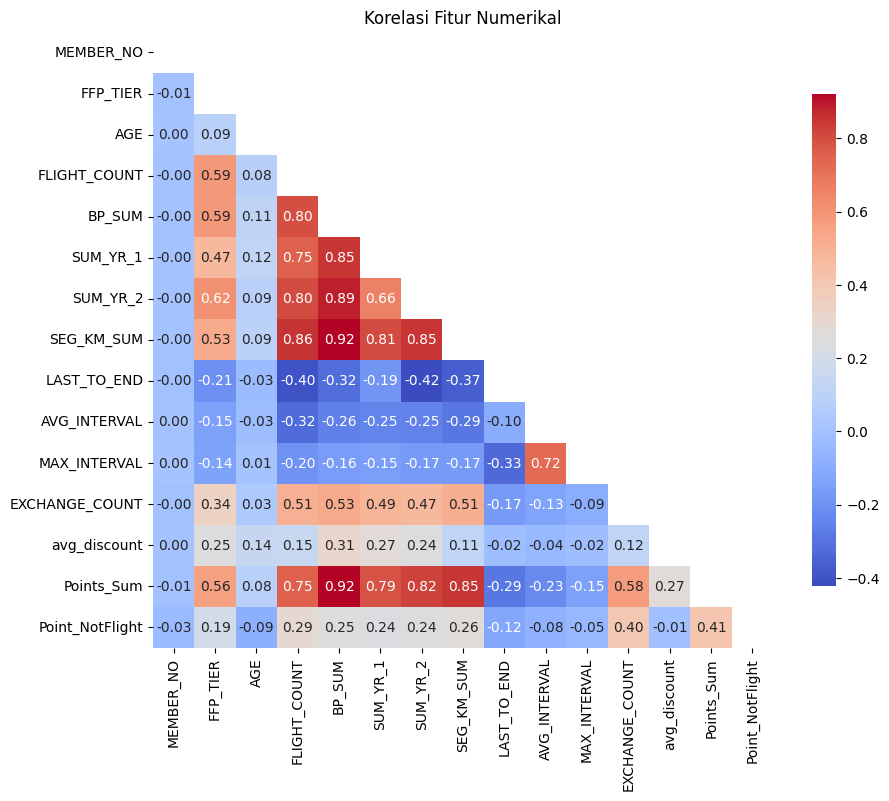
\includegraphics[width=0.7\textwidth]{gambar/heatmap.png}
    \caption{Heatmap dari fitur numerikal}
    \label{fig:heatmap}
\end{figure}

Dari heatmap tersebut, dapat dilihat bahwa beberapa fitur memiliki korelasi yang cukup tinggi yaitu 0.92 , seperti\texttt{SEG\_KM\_SUM} dan \texttt{BP\_SUM} , serta 0.86 untuk \texttt{SUM\_YR\_2} dan \texttt{BP\_SUM}. Hal ini menunjukkan bahwa fitur-fitur tersebut memiliki hubungan yang erat satu sama lain. Korelasi yang tinggi ini dapat mempengaruhi hasil clustering, kita tidak ingin menggunakan fitur yang memiliki multikollinearitas yang tinggi karena dapat menyebabkan masalah dalam interpretasi hasil clustering. Oleh karena itu, saya memutuskan untuk menghapus fitur \texttt{BP\_SUM} dari dataset, karena fitur ini memiliki korelasi yang tinggi dengan fitur lainnya. Namun sebelum membuang fitur tersebut, saya akan melakukan analisis lebih lanjut untuk memastikan bahwa fitur ini tidak memberikan informasi yang signifikan dalam proses clustering.

\subsubsection{Analisis Fitur Kategorikal}
% Analisis Fitur Kategorikal
Setelah melakukan analisis terhadap fitur numerikal, langkah selanjutnya adalah melakukan analisis terhadap fitur kategorikal. Fitur kategorikal adalah atribut yang memiliki nilai kategori atau label, seperti jenis kelamin, tier program, kota asal, dan provinsi asal. Dalam tugas ini, fitur kategorikal kurang relevan mengingat kita akan membuat model K means yang membutuhkan fitur numerikal. Oleh karena itu, kita akan membuang fitur kategorikal yang tidak relevan dari dataset. Fitur kategorikal yang akan dibuang antara lain:

\begin{enumerate}
    \item GENDER
    \item WORK\_CITY
    \item WORK\_PROVINCE
    \item WORK\_COUNTRY
\end{enumerate}

Selain karena fitur tersebut tidak relevan untuk model K means, fitur tersebut juga memiliki makna bisnis yang kurang signifikan dalam konteks clustering customer airline frequent flyer program. Oleh karena itu, fitur-fitur tersebut akan dihapus dari dataset untuk memastikan bahwa data yang digunakan untuk clustering hanya terdiri dari fitur-fitur yang relevan dan memberikan informasi yang signifikan.

\subsubsection{Insight}
% Insight
Setelah melakukan EDA, Agar dapat memberikan insight yang lebih dalam mengenai data, selain melakukan analisis terhadap fitur-fitur yang sekiranya relevan untuk clustering saya juga akan menggunakan fitur fitur yang tidak relevan untuk menggali insight. Dimana diharapkan fitur fitur tersebut dapat memberikan informasi yang lebih lengkap mengenai karakteristik customer airline frequent flyer program. Insight ini dapat dimanfaatkan untuk tim bisnis dalam mengambil keputusan yang lebih baik terkait strategi pemasaran, pengembangan produk, dan peningkatan layanan kepada pelanggan. 

Agar insight dapat digali dengan baik maka ada beberapa pertanyaan yang perlu dijawab, antara lain:

\begin{enumerate}
    \item Seberapa loyal member berdasarkan tier FFP?
    \item Apakah ada segmen umur yang memiliki frekuensi terbang tinggi?
    \item Apakah pelanggan dengan menukar poin dengan jumlah yang tinggi adalah mereka yang juga paling sering terbang?
\end{enumerate}

Untuk menjawab pertanyaan pertama tentang loyalitas member berdasarkan tier FFP, kita dapat menghitung jarak penerbangan customer pada setiap tier FFP. Gambar \ref{fig:ffp_tier} menunjukkan jarak penerbangan customer pada setiap tier FFP.

Dapat dilihat dari gambar tersebut bahwa tier FFP yang memiliki jarak penerbangan paling tinggi adalah tier 6, diikuti oleh tier 5, tier 4, dan seterusnya. Hal ini menunjukkan bahwa semakin tinggi tier FFP yang dimiliki oleh customer, semakin tinggi pula jarak penerbangan yang telah dilakukan. Hal ini dapat diartikan bahwa customer dengan tier FFP yang lebih tinggi cenderung lebih loyal terhadap program frequent flyer, karena mereka telah melakukan lebih banyak penerbangan dan mengumpulkan lebih banyak poin.

\begin{figure}[H]
    \centering
    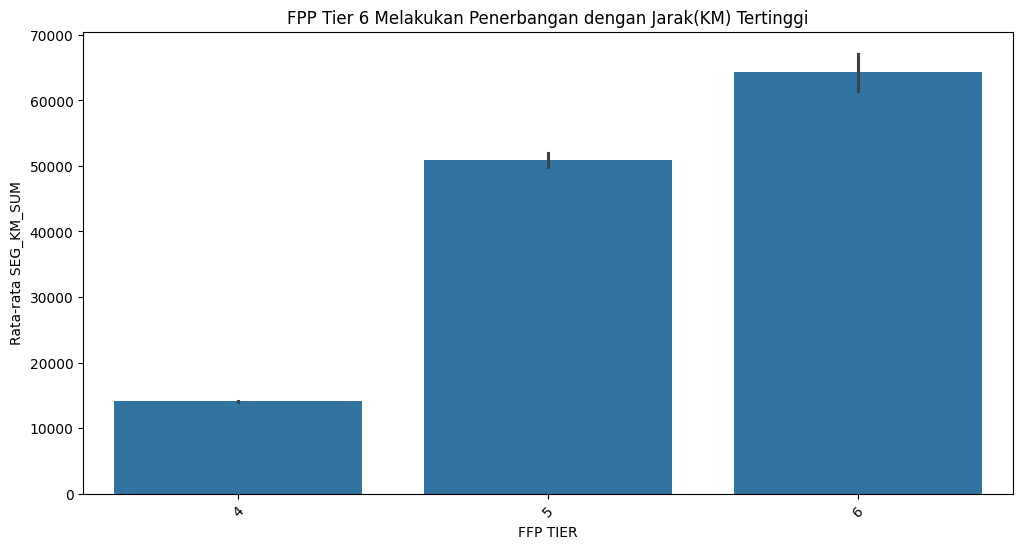
\includegraphics[width=0.7\textwidth]{gambar/fpp1.png}
    \caption{Jumlah customer pada setiap tier FFP}
    \label{fig:ffp_tier}
\end{figure}

Untuk menjawab pertanyaan kedua tentang segmen umur yang memiliki frekuensi terbang tinggi, kita dapat membuat histogram yang menunjukkan distribusi umur customer berdasarkan jumlah penerbangan yang telah dilakukan. Gambar \ref{fig:age_flight_count} menunjukkan distribusi umur customer berdasarkan jumlah penerbangan.

\begin{figure}[H]
    \centering
    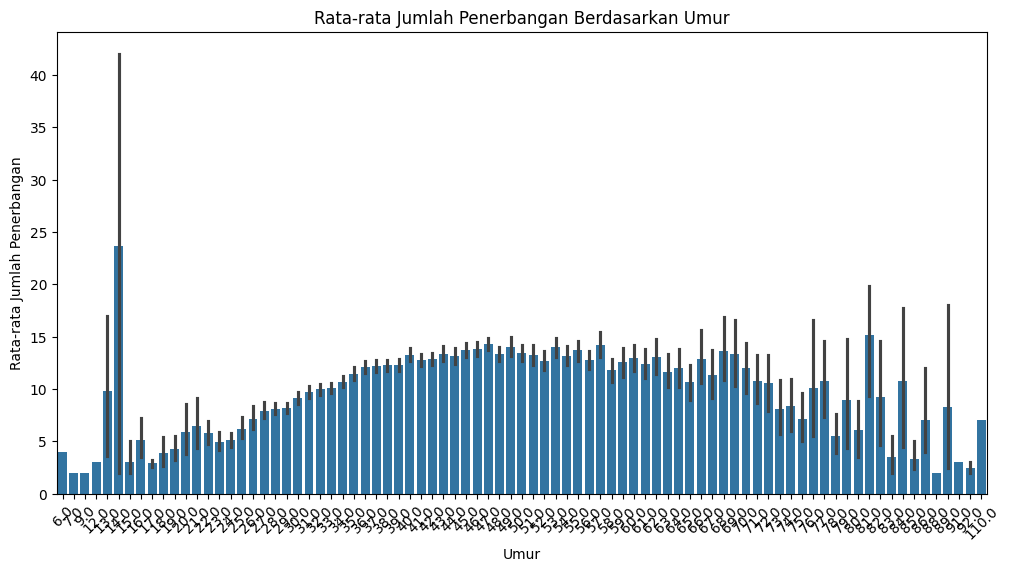
\includegraphics[width=0.7\textwidth]{gambar/umur.png}
    \caption{Distribusi umur customer berdasarkan jumlah penerbangan}
    \label{fig:age_flight_count}
\end{figure}

Dari histogram tersebut, dapat dilihat bahwa segmen umur yang memiliki frekuensi terbang tinggi adalah customer dengan umur antara 20 sampai 30 tahun. Hal ini menunjukkan bahwa customer dalam rentang umur tersebut cenderung lebih aktif dalam melakukan penerbangan dibandingkan dengan segmen umur lainnya. Namun dari histogram tersebut juga menunjukan bahwa umur 14 tahun adalah umur yang paling banyak melakukan penerbangan, hal ini mungkin disebabkan oleh anak dari orang tua yang memiliki frequent flyer program, sehingga anak tersebut dapat menggunakan poin dari orang tuanya untuk melakukan penerbangan.

Untuk menjawab pertanyaan ketiga tentang apakah pelanggan dengan menukar poin dengan jumlah yang tinggi adalah mereka yang juga paling sering terbang, kita dapat membuat histogram yang menunjukkan hubungan antara jumlah poin yang ditukar dengan jumlah penerbangan yang telah dilakukan. Gambar \ref{fig:points_flight_count} menunjukkan hubungan antara jumlah poin yang ditukar dengan jumlah penerbangan.

\begin{figure}[H]
    \centering
    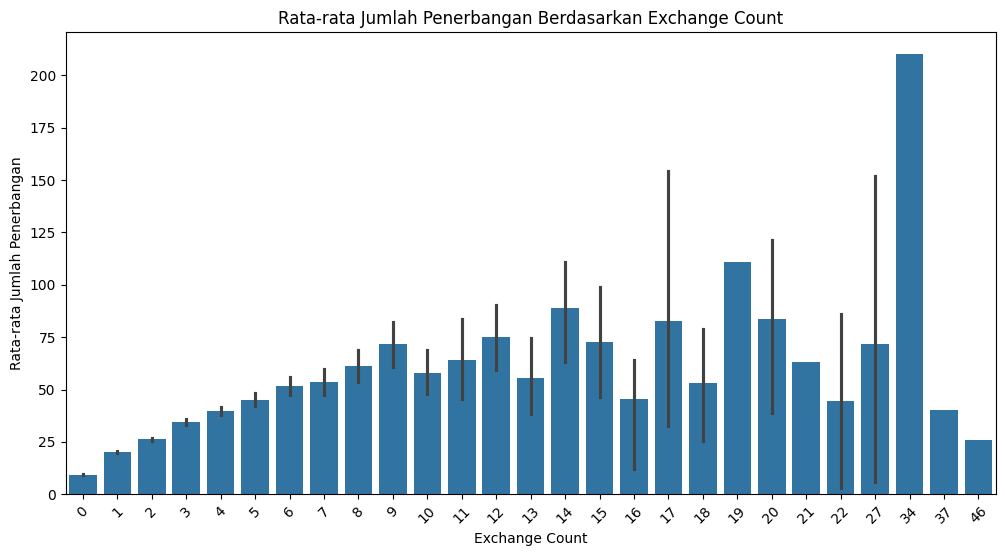
\includegraphics[width=0.7\textwidth]{gambar/exchange.png}
    \caption{Hubungan antara jumlah poin yang ditukar dengan jumlah penerbangan}
    \label{fig:points_flight_count}
\end{figure}

Dari histogram tersebut, dapat dilihat bahwa beberapa customer yang menukar poin dengan jumlah yang tinggi memiliki rata rata jumlah penerbangan terbanyak. Hal ini menunjukkan bahwa pelanggan yang sering terbang cenderung lebih aktif dalam menukar poin yang mereka miliki. Namun, ada juga beberapa customer yang menukar poin dengan jumlah yang tinggi tetapi memiliki jumlah penerbangan yang rendah. Hal ini mungkin disebabkan oleh beberapa faktor, seperti penggunaan poin untuk upgrade kelas penerbangan atau penukaran dengan barang.

\subsection{Preprocessing}
% Preprocessing
Setelah melakukan EDA dan mendapatkan insight yang lebih dalam mengenai data, langkah selanjutnya adalah melakukan preprocessing terhadap data yang akan digunakan untuk clustering. Preprocessing ini meliputi feature selection, normalisasi data, dan penanganan outliers. Proses ini bertujuan untuk memastikan bahwa data yang digunakan untuk clustering memiliki kualitas yang baik dan dapat memberikan hasil yang optimal.

\subsubsection{Feature Selection}
% Feature Selection
Feature selection adalah proses pemilihan fitur-fitur yang relevan untuk digunakan dalam clustering. Dalam tugas ini, saya memilih fitur-fitur yang dianggap relevan berdasarkan analisis EDA yang telah dilakukan sebelumnya. Namun karena dalam tugas ini kita akan menggunakan K-means, maka fitur yang digunakan harus berupa fitur numerikal.

Agar memiliki interpretasi yang baik pemilihan fitur haruslah didasari oleh RFM (Recency, Frequency, Monetary), dimana artinya fitur fitur tersebut haruslah mampu merepresentasikan seberapa sering customer melakukan penerbangan, seberapa lama customer sudah menjadi member, dan seberapa banyak uang yang telah dikeluarkan oleh customer. Berdasarkan hal tersebut, fitur-fitur yang dipilih untuk digunakan dalam clustering adalah sebagai berikut:

\begin{enumerate}
    \item \texttt{LAST\_TO\_END}: Jarak waktu antara penerbangan terakhir dengan pesanan penerbangan paling akhir. Ini menggambarkan Recency dari customer.
    \item \texttt{AVG\_INTERVAL}: Rata-rata jarak waktu antara penerbangan yang dilakukan oleh customer. Ini menggambarkan Frequency dari customer.
    \item \texttt{SUM\_YR\_1}: Total fare revenue yang dihasilkan oleh customer pada tahun pertama. Ini menggambarkan Monetary value dari customer.
\end{enumerate}

Sehingga dengan menggunakan fitur \texttt{LAST\_TO\_END}, \texttt{AVG\_INTERVAL}, dan \texttt{SUM\_YR\_1}, diharapkan dapat memberikan informasi yang cukup untuk melakukan clustering terhadap customer airline frequent flyer program. Fitur-fitur ini dipilih karena dianggap relevan dan dapat memberikan wawasan yang lebih dalam mengenai perilaku dan karakteristik customer. Target saya adalah dapat membentuk cluster yang dapat merepresentasikan segmen-segmen customer yang berbeda berdasarkan perilaku mereka dalam menggunakan layanan penerbangan. Adapun cluster tersebut adalah :

\begin{enumerate}
    \item Recency Rendah, Frequency Rendah, Monetary Tinggi merupakan Customer VIP.
    \item Recency Rendah, Frequency Rendah, Monetary Rendah merupakan Customer Active Frequent Low Spender.
    \item Recency Tinggi, Frequency Rendah, Monetary Rendah merupakan Lapsed Frequent Low Spender.
    \item Recency Rendah, Frequency Tinggi, Monetary Rendah merupakan Occasional Low Value.
\end{enumerate}

Sehingga hasil dari model clustering ini diharapkan dapat memberikan wawasan yang lebih dalam mengenai perilaku dan karakteristik customer airline frequent flyer program. Dengan demikian, perusahaan penerbangan dapat mengoptimalkan strategi pemasaran dan meningkatkan pengalaman pelanggan.

\subsubsection{Outlier Handling}
% Outlier Handling
Setelah melakukan feature selection, langkah selanjutnya adalah menangani outliers yang ada pada fitur-fitur yang telah dipilih. Outliers dapat mempengaruhi hasil clustering yang dihasilkan, sehingga perlu dilakukan penanganan untuk memastikan bahwa data yang digunakan untuk clustering lebih representatif. Dalam tugas ini, saya menggunakan metode IQR (Interquartile Range) untuk mengidentifikasi dan menangani outliers. 

Metode IQR adalah metode yang umum digunakan untuk mendeteksi outliers dengan cara menghitung rentang interkuartil (IQR) dari data. Rentang interkuartil adalah selisih antara kuartil ketiga (Q3) dan kuartil pertama (Q1). Outliers didefinisikan sebagai nilai yang berada di bawah Q1 - 1.5 * IQR atau di atas Q3 + 1.5 * IQR.

Gambar \ref{fig:outlier_handling} menunjukkan boxplot sebelum dilakukan penanganan outliers :

\begin{figure}[H]
    \centering
    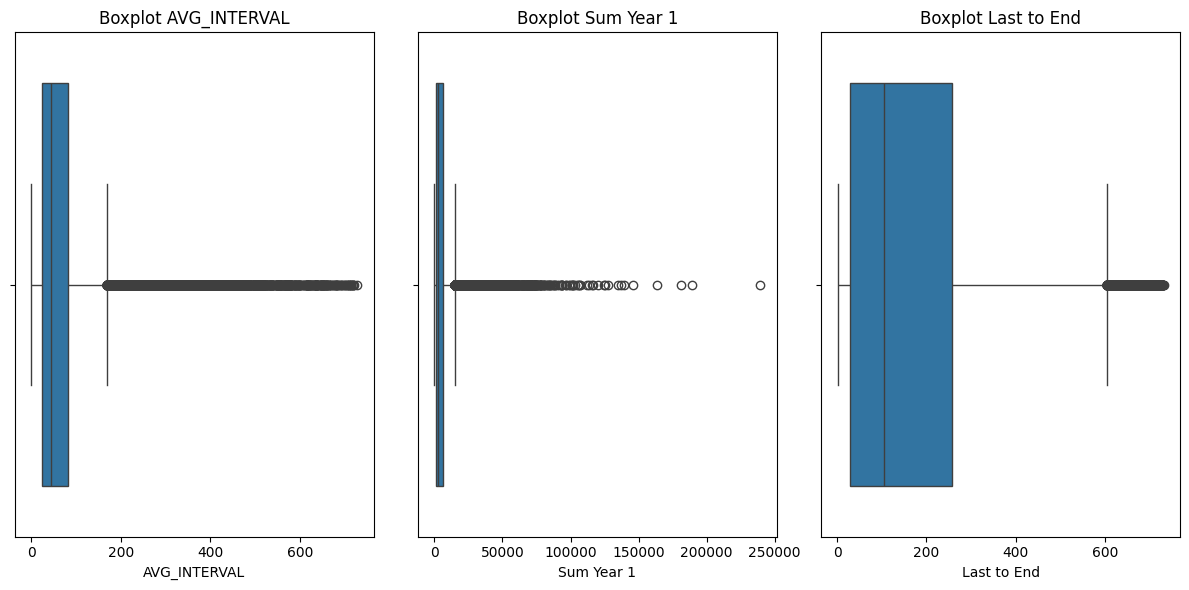
\includegraphics[width=0.7\textwidth]{gambar/outlier.png}
    \caption{Boxplot sebelum penanganan outliers}
    \label{fig:outlier_handling}
\end{figure}

Setelah melakukan penanganan outliers, saya akan membuat boxplot kembali untuk melihat apakah outliers telah berhasil diatasi. Gambar \ref{fig:outlier_handling_after} menunjukkan boxplot setelah dilakukan penanganan outliers :

\begin{figure}[H]
    \centering
    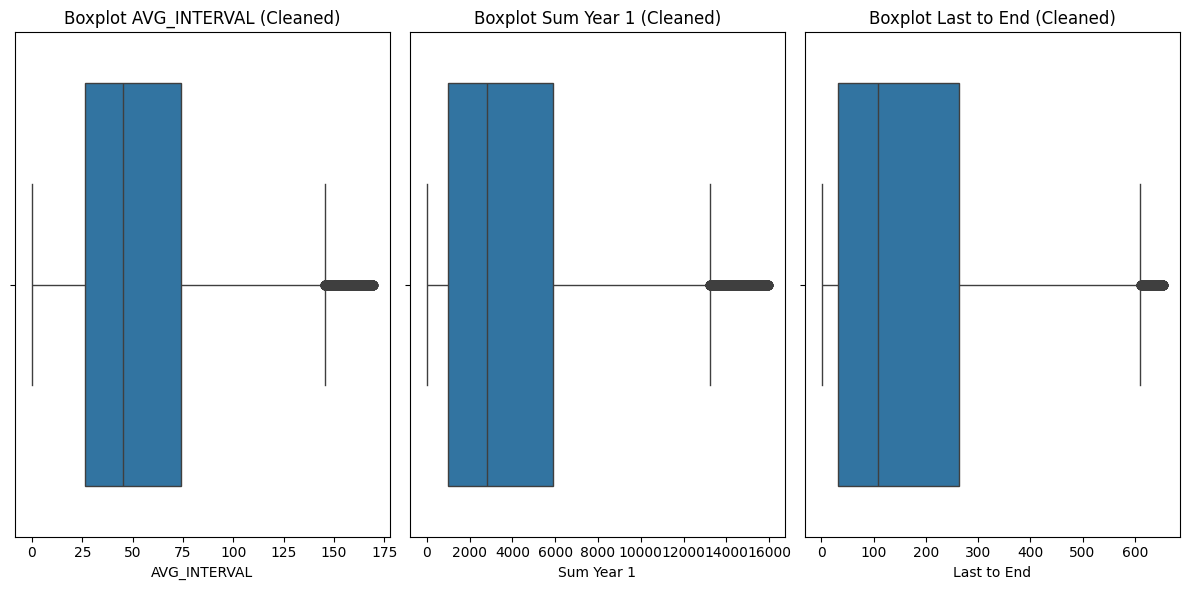
\includegraphics[width=0.7\textwidth]{gambar/clean.png}
    \caption{Boxplot setelah penanganan outliers}
    \label{fig:outlier_handling_after}
\end{figure}

Dari boxplot tersebut, dapat dilihat bahwa outliers telah berhasil diatasi, sehingga data yang digunakan untuk clustering menjadi lebih representatif. Penanganan outliers ini penting dilakukan untuk memastikan bahwa hasil clustering yang dihasilkan tidak dipengaruhi oleh nilai-nilai yang ekstrem.

\subsubsection{Standardisasi Data}
% Standardisasi Data
Setelah melakukan penanganan outliers, langkah selanjutnya adalah melakukan standardisasi data. Standardisasi data adalah proses mengubah skala fitur-fitur numerikal sehingga memiliki rata-rata 0 dan deviasi standar 1. Kita akan menggunakan StandardScaler dari library scikit-learn untuk melakukan standardisasi data. Standardisasi ini penting dilakukan karena K-means sensitif terhadap skala fitur, sehingga fitur-fitur yang memiliki skala yang berbeda dapat mempengaruhi hasil clustering yang dihasilkan.

\begin{lstlisting}[language=Python]
from sklearn.preprocessing import StandardScaler

scaler = StandardScaler()
df_scaled = df_cleaned.copy()
df_scaled[['AVG_INTERVAL', 'SUM_YR_1', 'LAST_TO_END']] = scaler.fit_transform(
    df_cleaned[['AVG_INTERVAL', 'SUM_YR_1', 'LAST_TO_END']])


# Print hasil standardisasi
    SUM_YR_1	LAST_TO_END	AVG_INTERVAL
84	2.264277	-0.684468	-0.579736
116	0.928944	-0.857778	-0.742002
121	-1.037080	-0.955987	-1.297966
.....
.....
\end{lstlisting}

Setelah melakukan standardisasi, data yang digunakan untuk clustering sudah siap. Data ini akan digunakan sebagai input untuk model K-means yang akan dibangun pada tahap selanjutnya. Dengan data yang telah distandarisasi, diharapkan hasil clustering yang dihasilkan akan lebih akurat dan representatif terhadap karakteristik customer airline frequent flyer program.






\newpage

\section{Pengujian dan analisis}

\subsection{Pengujian Sistem}

\newpage
\section{Kesimpulan dan Saran}

\end{document}